\chapter{Realisierung Objekt Erkennung}\label{kap:object_det}

\section{Datensatz}\label{sec:dataset}

Um ein Deep Learning Modell richtig trainieren zu können, 
wird eine große Menge an gelabelten Trainingsdaten benötigt.
Handelt es sich dabei um ein, wie in Abschnitt
\ref{sec:related_work} beschriebenen  Modell zur Objekterkennung
müssen die Labels neben der Klasse, auch die Koordinaten, 
die angeben wo sich das Objekt im Bild befindet. 
Indem die, sogenannten Bouning Boxes, mit traininert werden, 
kann das Modell auch die Lokalisierung der Objekte vorhersagen.
Die Trainingsdaten können entweder selber erstellt, oder 
aus frei zugänglichen Datensätzen wie z.B. \textit{ImageNet}, 
\textit{COCO}, oder \textit{OpenImages}
aus dem Internet heruntergeladen werden.

Für die Arbeit wurden aus dem Open Source Dataset
\textit{OpenImages} von Google
\cite{kuznetsovaOpenImagesDataset2018}, 
welches 600 gelabelte Klassen enthällt, 
die 9 Klassen \textit{Brown bear, Deer, Fox, Goat, 
Hedgehog, Owl, Rabbit, Raccoon} und \textit{Squirrel}
heruntergeladen und für das Training verwendet.
Für die Evaluierung des Trainings wurde der 
Datensatz in ein Trainings, einen Validierung und einen 
Testset aufgeteilt, mit dem Verhälltnis 80\%, 10\%, 10\%.
Je Klasse variierte die Anzahl an Bildern zwischen 200 und 
2000, wudurch die in Abbildung \ref{fig:histo_ohne_aug}
dargestellte unausgeglichenheit der Klassen zustande kam.
Um diese auszugleichen, wurden die Date, wie im nächsten Abschnitt 
genauer erklärt wird, so augmentiert, das je Klasse 3000 Bilder 
vorhanden waren, was zu einer in Abbildung \ref{fig:histo_mit_aug}
dargestellten verteilung der Klassen führte.

\vspace{1cm}
\begin{minipage}{0.5\textwidth}
    \centering
    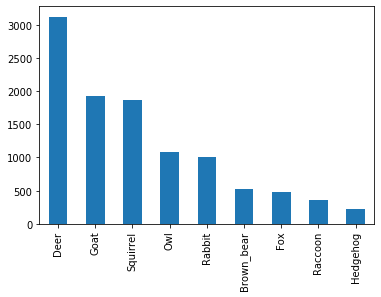
\includegraphics[width=0.9\textwidth]{class_distro.png}
    \captionof{figure}{ohne aug}
    \label{fig:histo_ohne_aug}
\end{minipage}
\begin{minipage}{0.5\textwidth}
    \centering
    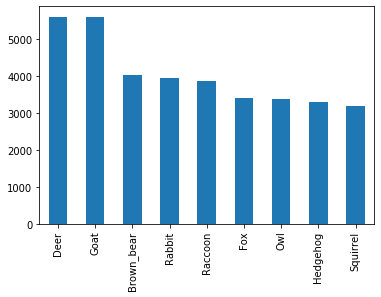
\includegraphics[width=0.9\textwidth]{class_distro_aug.png}
    \captionof{figure}{mit aug}
    \label{fig:histo_mit_aug}
\end{minipage}
\vspace{1cm}

Der Grund dafür, dass in den Histogrammen mehr Klassen,
als es tatsächlich Bilder 
waren angezeigt werden, kommt daher, dass 
sich häufig mehrere Tiere der selben Klasse in einem Bild 
befinden.
Ein weiterer Grund für die Augmentierung der Daten war 
die vorsogliche Maßnahme gegen Overfitting.




\subsection{Augmentierung}\label{subsec:augmentation}


Das augmentieren von Bilddaten für Deep Learning, 
ist eine effektive Technik, durch künstliches generieren
neuer Daten aus den vorhandenen, um Overfitting zu
verhindern und Inbalancen der Klassen untereinander auszugleichen.
Die vermehrung der Daten erfolg dabei in dem die Bilder 
geometrischen Transformationen oder manipulationen der Pixelwerte 
unterzogen werden.

Die Augmentierung des OpenImages Datensatzes wurde mithilfe 
eines Pyhton Scripts, welches die Library \textit{imgaug} \cite{imgaug}
verwendet, durchgeführt.
Dabei wurde je zu augmentierendem Bild eine geometrische und 
eine Pixel Transformation angewendet.
Diese wurden zufällig aus einer Auswahl an Augmentern, 
angewendetet.

Folgend ist ein Codeausschschnitt des Python Scripts dargestellt, 
welcher die verwendeten Augmentierungstechniken zeigt.


\begin{lstlisting}[language=Python]

    color_augmenters = [
        iaa.Dropout(p=(0, 0.1)),
        iaa.CoarseDropout((0.01, 0.05), size_percent=0.1),
        iaa.Multiply((0.5, 1.3), per_channel=(0.2)),
        iaa.GaussianBlur(sigma=(0, 5)),
        iaa.AdditiveGaussianNoise(scale=((0, 0.2*255))),
        iaa.ContrastNormalization((0.5, 1.5)),
        iaa.Grayscale(alpha=((0.1, 1))),
        iaa.ElasticTransformation(alpha=(0, 5.0), sigma=0.25),
        iaa.PerspectiveTransform(scale=(0.15)),
        iaa.MultiplyHueAndSaturation((0.7))
    ]

    geometric_augmenters = [
        iaa.Affine(scale=((0.6, 1.2))),
        iaa.Affine(translate_percent=(-0.3, 0.3)),
        iaa.Affine(shear=(-25, 25)),
        iaa.Affine(translate_percent={"x": (-0.3, 0.3), "y": (-0.2, 0.2)}),
        iaa.Fliplr(1),
        iaa.Affine(scale={"x": (0.6, 1.4), "y": (0.6, 1.4)})
    ]
    
\end{lstlisting}

In Abbildung \ref{fig:augmentierung} sind beispielhaft 9 dieser 
zufällig augmentierten Bilder für die Klasse Fuchs dargestellt.


\begin{figure}[H]
    \centering
    \label{fig:augmentierung}
    \includegraphics[width=0.9\columnwidth]{Bilder/augmentierung.png}
    \caption{Anwendung von Augmentierungstechniken}
\end{figure}





\section{Training}

Das Training der Deep Learning Modelle erfolgte mithilfe 
des Frameworks Tensorflow, welches auch von 
Open Vino für den Neural Compute Stick uterstütz wird.
Dabei wurde eine speziell für Object Detection 
entwickelte Api von Tensorflow verwendet.

Um unabhängig von der leistungsfähigkeit der GPU des eigenen 
Rechners zu sein, wurde das Training in der Cloudbasierten Virtual 
Machine \textit{Google Colab} \cite{colab} durchgeführt, welche kostenlos eine für 
Deep Learning geeignete GPU zur verfügung stellt.



\subsection{Tensorflow Object Detection Api}



Die Tensorflow Object Detection Api ist unter den Research Modellen
\cite{tfobjdet} des offiziellen Tensorflow Repository auf GitHub zu
finden und enthällt implementierungen einiger gängiger Object Detectin
Modelle mit vortrainierten gewichten zur Feature Extraction.
Für die Arbeit wurde die im Abschnitt \ref{sec:related_work} 
erläuterten Architekturen \textit{Single Shot Detector (SSD)}
und \textit{Faster R-CNN} verwendet.
Beim SSD wurde das \textit{MobilenetV2} sowie das \textit{InceptionV2} 
als Basis CNN verwendet.
Bei Faster R-CNN nur \textit{InceptionV2}, da hierfür das MobilenetV2 
nicht verfügbar war.
Weitere Basis CNN sind unter Anderem das Resudial Network, welche jedoch 
sehr Rechenaufwendig und nicht für den Neural Compute Stick 
kompatibel ist.

Die Festlegung der Parameter für die Modelle kann dabei 
in einer Konfigurationsdatei vorgenommen werde.


Um die Modelle trainieren zu können, mussten zunächst die 
Trainingsdaten in das binary Dateiformate TFRecords umgewandelt 
werden, welches die Api verwendet. Dieses ist eine Serialisierte 
darstellung der Bilder und Labels als Protocol Buffer welche einen 
schnelleren Zugriff auf die Daten ermöglicht.

Nach herunterladen des Modellund festlegen einiger Parameter was in 
einem Jupyter Notebook der Colab VM erfolgte, konnte das Training 
gestatret werden. 

Das erfolgte über einen Command dem die TfRecord Files als Argument 
übergebun wurden. 
Die Trainierten Gewichte wurden während des Trainings regelmäßig abgespeichert.

Mithilfe das Evaluierungstools Tensorboard konnte der Trainingsfortschrit 
mitverfolgt und ausgewertet werden.


\subsection{Trainingsworkflow}

Durch die in Tensorboard visualisierte beobachtung der 
Trainingsverläufe, konnten so schon während des traings fehlerhafte 
Einstellung der Trainingskonfigurarion festgestellt und korrigiert 
werden.

So ergibt sich der in ... dargestellte Workflow, in dem 
durch unterschiedliche Konfigurationen der für das Training 
benötigten Schritte, das Optimalste Endergebniss erzielt 
werden kann.


Anpasungen die für die trainierten Modelle SSD und Faster 
R-CNN vorgenommen wurden bezogen sich auf unterschiedliche 
Augmentierung der Trainingsdaten, sowie verschiedene 
einstellungen der Hyperparameter.


% \begin{figure}[H]
%     \centering
%     \def\svgwidth{0.7\textwidth}
%     
\tikzstyle{process} = [rectangle, fill=blue!20, node distance=4cm, minimum width=1.5cm, minimum height=0.8cm, text centered, draw=black]
\tikzstyle{arrow} = [thick,->,>=stealth]
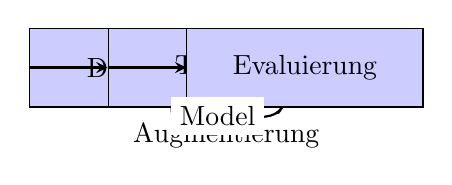
\begin{tikzpicture}[scale=0.4]
      \node (data)      [process]                   {Datensatz};
      \node (train)      [process, right of=data]      {Training};
      \node (eval)      [process, right of=train]      {Evaluierung};
    \draw[arrow] (data) -- (train);
    \draw[arrow] (train) -- (eval);
  \draw[arrow] (eval) edge[bend left=60] node [centered, fill=white!30] {Augmentierung} (data);
  \draw[arrow] (eval) edge[bend left=60] node [left, fill=white!30] {Model} (train);
\end{tikzpicture}

% \begin{tikzpicture}[scale=0.4]

%   \begin{scope}[node distance=3cm]

%    \node (data)      [process]                   {Datensatz};
%    \node (prep)      [process, right of=data]      {Aufbereitung};
%    \node (model)      [process, right of=prep]      {Model};
%    \node (train)      [process, right of=model]      {Training};
%    \node (eval)      [process, right of=train]      {Evaluierung};

%   \end{scope}

%  \draw[arrow] (data) -- (prep);
%  \draw[arrow] (prep) -- (model);
%  \draw[arrow] (model) -- (train);
%  \draw[arrow] (train) -- (eval);
 

% \draw[arrow] (eval) edge[bend left=60] node [left, fill=white!30] {ändern} (data);
% \draw[arrow] (eval) edge[bend left=60] node [left, fill=white!30] {augment} (prep);
% \draw[arrow] (eval) edge[bend left=60] node [left, fill=white!30] {ändern} (model);
% \draw[arrow] (eval) edge[bend left=60] node [left, fill=white!30] {Parameter} (train);

 
% \end{tikzpicture}

%     \caption{Trainingsworkflow}
%     \label{fig:train_workflow}
% \end{figure}

% \vspace{1cm}

\begin{figure}[H]
    \centering
    
\tikzstyle{process} = [rectangle, fill=blue!20, node distance=4cm, minimum width=1.5cm, minimum height=0.8cm, text centered, draw=black]
\tikzstyle{arrow} = [thick,->,>=stealth]
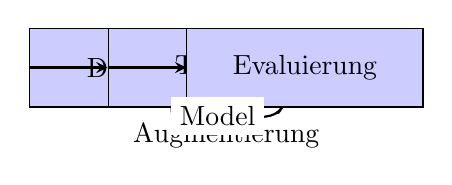
\begin{tikzpicture}[scale=0.4]
      \node (data)      [process]                   {Datensatz};
      \node (train)      [process, right of=data]      {Training};
      \node (eval)      [process, right of=train]      {Evaluierung};
    \draw[arrow] (data) -- (train);
    \draw[arrow] (train) -- (eval);
  \draw[arrow] (eval) edge[bend left=60] node [centered, fill=white!30] {Augmentierung} (data);
  \draw[arrow] (eval) edge[bend left=60] node [left, fill=white!30] {Model} (train);
\end{tikzpicture}

% \begin{tikzpicture}[scale=0.4]

%   \begin{scope}[node distance=3cm]

%    \node (data)      [process]                   {Datensatz};
%    \node (prep)      [process, right of=data]      {Aufbereitung};
%    \node (model)      [process, right of=prep]      {Model};
%    \node (train)      [process, right of=model]      {Training};
%    \node (eval)      [process, right of=train]      {Evaluierung};

%   \end{scope}

%  \draw[arrow] (data) -- (prep);
%  \draw[arrow] (prep) -- (model);
%  \draw[arrow] (model) -- (train);
%  \draw[arrow] (train) -- (eval);
 

% \draw[arrow] (eval) edge[bend left=60] node [left, fill=white!30] {ändern} (data);
% \draw[arrow] (eval) edge[bend left=60] node [left, fill=white!30] {augment} (prep);
% \draw[arrow] (eval) edge[bend left=60] node [left, fill=white!30] {ändern} (model);
% \draw[arrow] (eval) edge[bend left=60] node [left, fill=white!30] {Parameter} (train);

 
% \end{tikzpicture}

    \caption{Trainingsworkflow}
    \label{fig:train_workflow}
\end{figure}

Die Ergebnisse der jeweiligen Ansätze werden im nächsten Kapitel diskutiert.


\section{Inferenz}\label{sec:inferenz}

Die Anwendung eines fertig trainierten Modells für 
neue Inputdaten, wird als Inferenz bezeichnet.
Zur Ausführung dieser auf dem NCS2, wird wie in 
den Grundlagen beschriebene das Toolkit \textit{OpenVino}
von Intel verwendet.

Dafür musste zunächst der trainierte Tensorflow Graph 
exportiert, d.h. die aktuellen Werte der Gewichte 
konstant gesetzt werden.

Mit dem ModelOptimizer, der ebnfalls im OpenVino 
Toolkit enthalten war konnte das Tensorflow Modell 
in die Intermediate Representation (IR), bestehend 
aus einer xml und einer bin Datei konvertiert werden.


Diese können nun von der InferecneEgine zur Inferenz weiter 
verwendet werden.


\subsection*{InferecneEgine}


Die für die Inferenz eines Modells im IR Formal 
auf dem NCS2 notwendigen Schritte, welche die
 InferecneEgine ausführt, sind in Abbildugn
\ref{fig:inger_engine_workflow} schematisch dargestellt.

Daneben ist jeweils (teils vereinfacht) die entsprechende 
Codezeile in Python abgebildet.

Zunächst muss das Zielgerät spezifiziert (\textit{HW Plugin laden})
und das Model anhand der IR Dateien definiert werden
(\textit{Model IR einlesen}), um daraus 
das Ausführbare Model erzugen zu können (\textit{executable Model}).

\textit{In-und Outputblob} sind die diemensionen welche
das Model in den In-und Output Schichten hat
und an die das Array des zu inferierenden 
Bilds angepasst werden müssen, was im Schritt 
\textit{preprocess Input} geschieht.

Nachdem die Inferenz abschossen ist, können die 
ergebnisse weter verarbeitet werden, handelt es sich 
die Inferenz eines Videos oder Kamera Streams, 
werden die Schritte preprocess, Inferenz und 
process Output in einer Schleife wiederholt.


\begin{minipage}{0.30\textwidth}
    \centering
    
\tikzstyle{process} = [rectangle, fill=blue!20, minimum width=3cm, minimum height=1cm, text centered, draw=black]
\tikzstyle{arrow} = [thick,->,>=stealth]

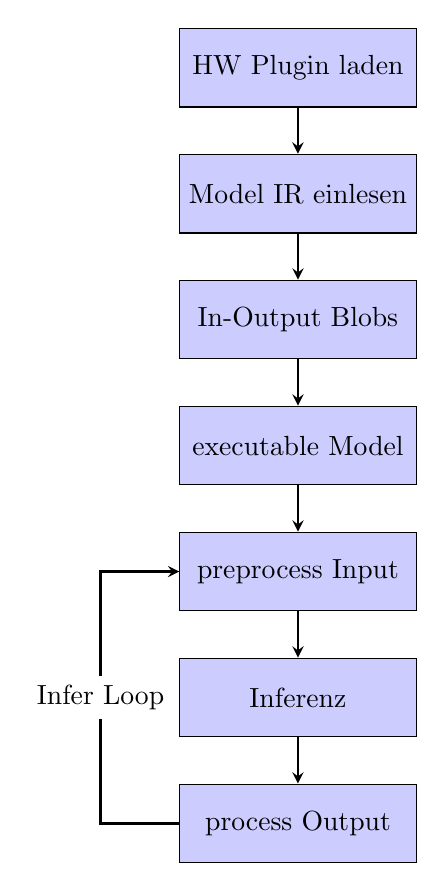
\begin{tikzpicture}[node distance=1.6cm]
    \node (hw)      [process]                   {HW Plugin laden};
    \node (ir)      [process, below of=hw]      {Model IR einlesen};
    \node (io)      [process, below of=ir]      {In-Output Blobs};
    \node (execNet) [process, below of=io]      {executable Model};
    \node (prepIn)  [process, below of=execNet] {preprocess Input};
    \node (infer)   [process, below of=prepIn]  {Inferenz};
    \node (procOut) [process, below of=infer]   {process Output};

    \draw [arrow] (hw) -- (ir);
    \draw [arrow] (ir) -- (io);
    \draw [arrow] (io) -- (execNet);
    \draw [arrow] (execNet) -- (prepIn);
    \draw [arrow] (prepIn) -- (infer);
    \draw [arrow] (infer) --  (procOut);

    \draw [arrow] (procOut.west) -- +(-1,0) |- node[pos=0.25, fill=white!30] {Infer Loop} (prepIn);

    
\end{tikzpicture}

    \captionof{figure}{}
    \label{fig:inger_engine_workflow}
\end{minipage}
\begin{minipage}{0.70\textwidth}

%\begin{python}
\begin{lstlisting}[language=Python]

    plugin = IEPlugin(device='MYRIAD')

        
    net = IENetwork(model_xml, model_bin)
        
    
    input_blob  = net.inputs
    output_blob = net.outputs
        

    exec_net = plugin.load_network(net, n_req)
        
    while True:

        image = preprocess(capture) # hwc -> nchw
        
        
        res = exec_net.infer({input_blob : image})
        

        res = res[output_blob] #
        
        
\end{lstlisting}
%\end{python}
\vspace{1.5cm}
\end{minipage}

% transform:
% # capture dims zu input blob dims transformieren
% # img_h, img_w, img_c -> blob_n, blob_c, blob_h, blob_w

Die Form des Inferenz Ergebnisses hängt von der 
Art des verwendeten Deep Learning Modells ab, welche 
z.B. Image Classification, ObjectDetection, oder Instance
Segmentation sein können.

Für Object Detection Modelle enthällt das Ergebnis Datenstrukturen, 
welche den Index der Klassen, zugehörige Wahrscheinlichkeit, 
sowie Boxkoordinate der geschätzen Objekte im Bild enthalten.

Indem man für alle Schätzungen die in einem Bild gemacht werden 
einen Threshhold für die Wahrscheinlichkeit festlegt (zb. 0,7),
könenn die sinnvollen Ergebnisse herausgefiltert werdsen.

Zur veranschaulichung können die Koordinaten dann 
als Bounding Box in das Inferierte Bild gezeichnet werden.
